

\begin{figure}

  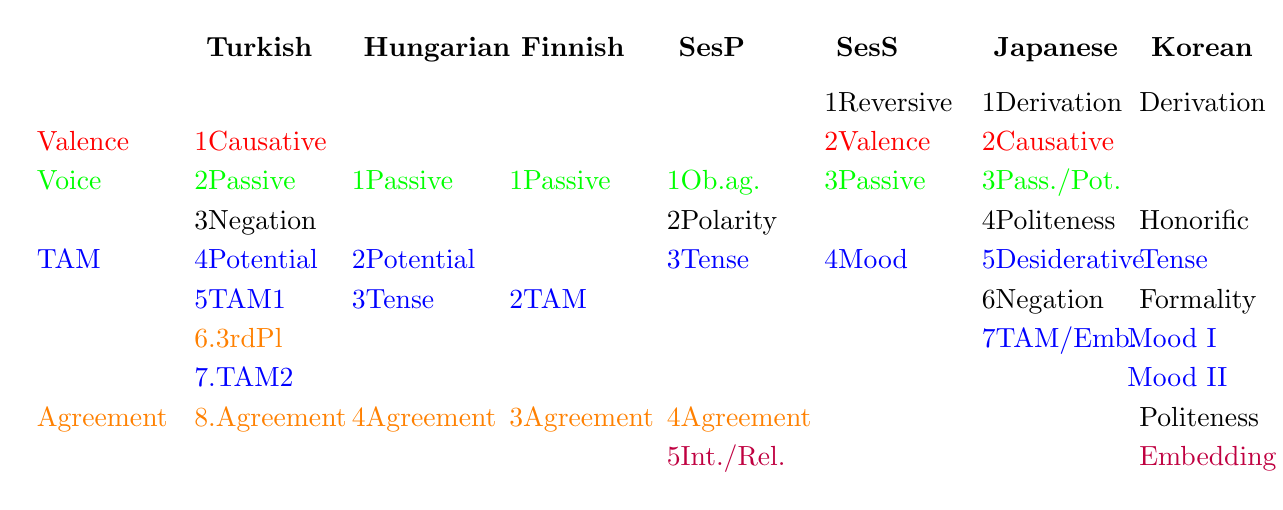
\begin{tikzpicture}[%
% common options for blocks:
block/.style = {draw, fill=blue!30, align=center, anchor=west,
            minimum height=0.65cm, inner sep=0},
% common options for the circles:
ball/.style = {circle, draw, align=center, anchor=north, inner sep=0}]
%\node[rectangle,text width=1.2cm,anchor=base] (A0) at (1,-0.3) {Real};

%\node[rectangle,text width=5cm,anchor=left, color=red, fill=red, opacity=0.1] (A02) at (1,-1.5) {};

%\node[rectangle,text width=1.2cm,anchor=base] (A1) at (1,-1.0) {1Derivation};
\node[rectangle,text width=1.2cm,anchor=base, color=red] (A2) at (1,-1.5) {Valence};
\node[rectangle,text width=1.2cm,anchor=base, color=green] (A3) at (1,-2.0) {Voice};
\node[rectangle,text width=1.2cm,anchor=base,color=blue] (A4) at (1,-3) {TAM};
%\node[rectangle,text width=1.2cm,anchor=base,color=blue] (A4) at (1,-3.5) {Tense};
%\node[rectangle,text width=1.2cm,anchor=base,color=blue] (A4) at (1,-4) {Mood};
\node[rectangle,text width=1.2cm,anchor=base,color=orange] (A4) at (1,-5) {Agreement};

% Turkish
\node[rectangle,text width=0.9cm,anchor=base] (B0) at (3,-0.3) {\textbf{Turkish}};
\node[rectangle,text width=1.2cm,anchor=base,color=red] (B1) at (3,-1.5) {1Causative};
\node[rectangle,text width=1.2cm,anchor=base,color=green] (B2) at (3,-2) {2Passive};
\node[rectangle,text width=1.2cm,anchor=base] (B3) at (3,-2.5) {3Negation};
\node[rectangle,text width=1.2cm,anchor=base,color=blue] (B4) at (3,-3) {4Potential};
\node[rectangle,text width=1.2cm,anchor=base,color=blue] (B4) at (3,-3.5) {5TAM1};
\node[rectangle,text width=1.2cm,anchor=base,color=orange] (B4) at (3,-4) {6.3rdPl};
\node[rectangle,text width=1.2cm,anchor=base,color=blue] (B4) at (3,-4.5) {7.TAM2};
\node[rectangle,text width=1.2cm,anchor=base,color=orange] (B4) at (3,-5) {8.Agreement};

% Hungarian
\node[rectangle,text width=0.9cm,anchor=base] (B0) at (5,-0.3) {\textbf{Hungarian}};
\node[rectangle,text width=1.2cm,anchor=base,color=green] (B2) at (5,-2) {1Passive};
\node[rectangle,text width=1.2cm,anchor=base,color=blue] (B4) at (5,-3) {2Potential};
\node[rectangle,text width=1.2cm,anchor=base,color=blue] (B4) at (5,-3.5) {3Tense};
\node[rectangle,text width=1.2cm,anchor=base,color=orange] (B4) at (5,-5) {4Agreement};


% Finnish
\node[rectangle,text width=0.9cm,anchor=base] (B0) at (7,-0.3) {\textbf{Finnish}};
\node[rectangle,text width=1.2cm,anchor=base,color=green] (B2) at (7,-2) {1Passive};
\node[rectangle,text width=1.2cm,anchor=base,color=blue] (B4) at (7,-3.5) {2TAM};
\node[rectangle,text width=1.2cm,anchor=base,color=orange] (B4) at (7,-5) {3Agreement};

% Sesotho Prefixes
\node[rectangle,text width=0.9cm,anchor=base] (B0) at (9,-0.3) {\textbf{SesP}};
\node[rectangle,text width=1.2cm,anchor=base,color=green] (B2) at (9,-2) {1Ob.ag.};
\node[rectangle,text width=1.2cm,anchor=base] (B4) at (9,-2.5) {2Polarity};
\node[rectangle,text width=1.2cm,anchor=base,color=blue] (B4) at (9,-3) {3Tense};
\node[rectangle,text width=1.2cm,anchor=base,color=orange] (B4) at (9,-5) {4Agreement};
\node[rectangle,text width=1.2cm,anchor=base,color=purple] (B4) at (9,-5.5) {5Int./Rel.};

% Sesotho Suffixes
\node[rectangle,text width=0.9cm,anchor=base] (B0) at (11,-0.3) {\textbf{SesS}};
\node[rectangle,text width=1.2cm,anchor=base] (B2) at (11,-1) {1Reversive};
\node[rectangle,text width=1.2cm,anchor=base,color=red] (B2) at (11,-1.5) {2Valence};
\node[rectangle,text width=1.2cm,anchor=base,color=green] (B2) at (11,-2) {3Passive};
\node[rectangle,text width=1.2cm,anchor=base,color=blue] (B4) at (11,-3) {4Mood};



% Japanese
\node[rectangle,text width=0.9cm,anchor=base] (B0) at (13,-0.3) {\textbf{Japanese}};
\node[rectangle,text width=1.2cm,anchor=base] (B2) at (13,-1) {1Derivation};
\node[rectangle,text width=1.2cm,anchor=base,color=red] (B2) at (13,-1.5) {2Causative};
\node[rectangle,text width=1.2cm,anchor=base,color=green] (B2) at (13,-2) {3Pass./Pot.};
\node[rectangle,text width=1.2cm,anchor=base] (B4) at (13,-2.5) {4Politeness};
\node[rectangle,text width=1.2cm,anchor=base,color=blue] (B4) at (13,-3) {5Desiderative};
\node[rectangle,text width=1.2cm,anchor=base] (B4) at (13,-3.5) {6Negation};
\node[rectangle,text width=1.2cm,anchor=base,color=blue] (B4) at (13,-4) {7TAM/Emb.};

% Korean
\node[rectangle,text width=0.9cm,anchor=base] (B0) at (15,-0.3) {\textbf{Korean}};
\node[rectangle,text width=1.2cm,anchor=base] (B2) at (15,-1.0) {Derivation};
\node[rectangle,text width=1.2cm,anchor=base] (B4) at (15,-2.5) {Honorific};
\node[rectangle,text width=1.2cm,anchor=base,color=blue] (B4) at (15,-3) {Tense};
\node[rectangle,text width=1.2cm,anchor=base] (B4) at (15,-3.5) {Formality};
\node[rectangle,text width=1.5cm,anchor=base,color=blue] (B4) at (15,-4.0) {Mood I};
\node[rectangle,text width=1.5cm,anchor=base,color=blue] (B4) at (15,-4.5) {Mood II};
\node[rectangle,text width=1.2cm,anchor=base] (B4) at (15,-5) {Politeness};
\node[rectangle,text width=1.2cm,anchor=base,color=purple] (B4) at (15,-5.5) {Embedding};


%\draw[->] (A1.east) to (B1.west);
%\draw[->] (A2.east) to (B2.west);
%\draw[->] (A3.east) to (B3.west);
%\draw[->] (A4.east) to (B4.west);
\end{tikzpicture}

%    \centering
%\begin{tabular}{l||l|l|l|l|l|l|llll}
%                    & Turkish & Hungarian & Finnish  & Sesotho Pref.     & Ses Suff. & Japanese & Korean\\ \hline\hline
%Derivation          &  &         &          &               & Reversive & suru    & ha,i\\ \hline
%Valence             &  Causative &         &           & Object marker & Valence & Causative\\ \hline
%Voice               & Passive & Passive    & Passive     &               & Passive & Passive\\ \hline
%TAM, Pol.           & Negation  &   Potential  &   Tense/Asp &    Negation &  Politeness &      Potential        & Honorific \\
%                    & Potential & Tense        &    Mood     &     Tense   &    Mood     &   Honorific  &    Tense       \\
%                    &   TAM1    &          &                &         &                  & Tense/Aspect & Formality \\
%                    & lar       &          &           &  & & Negation & Mood I\\
%                    & TAM2         &           &               &          &       &      &  Mood II \\ \hline
%Agreement           & Agreement & Agreement & Agreement & Agreement \\ \hline
%\textit{Other}               & Formality          & Clitic    &              & Int/Rel &      &        & Politeness \\
%                    &           &     &              &  &          &    & Conj \\
%\end{tabular}

\mhahn{TODO make this visually more appealing}

    \caption{Morpheme ordering across the six languages in our sample, matched with four universal categories (left).}
    \label{tab:examples-verbs}
\end{figure}




\begin{figure}
\begin{tabular}{ccccccc}
\textsc{Finnish} & \textsc{Hungarian} & \textsc{Turkish} \\
\begin{minipage}{.3\textwidth}
    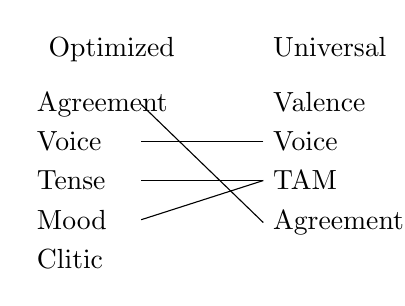
\begin{tikzpicture}[%
% common options for blocks:
block/.style = {draw, fill=blue!30, align=center, anchor=west,
            minimum height=0.65cm, inner sep=0},
% common options for the circles:
ball/.style = {circle, draw, align=center, anchor=north, inner sep=0}]
\node[rectangle,text width=1.2cm,anchor=base] (A0) at (4,-0.3) {Universal};
\node[rectangle,text width=0.9cm,anchor=base] (B0) at (1,-0.3) {Optimized};
\node[rectangle,text width=1.2cm,anchor=base] (A1) at (4,-1.0) {Valence};
\node[rectangle,text width=1.2cm,anchor=base] (A2) at (4,-1.5) {Voice};
\node[rectangle,text width=1.2cm,anchor=base] (A3) at (4,-2.0) {TAM};
\node[rectangle,text width=1.2cm,anchor=base] (A4) at (4,-2.5) {Agreement};
\node[rectangle,text width=1.2cm,anchor=base] (B1) at (1,-1.0) {Agreement};
\node[rectangle,text width=1.2cm,anchor=base] (B2) at (1,-1.5) {Voice};
\node[rectangle,text width=1.2cm,anchor=base] (B3) at (1,-2.0) {Tense};
\node[rectangle,text width=1.2cm,anchor=base] (B4) at (1,-2.5) {Mood};
\node[rectangle,text width=1.2cm,anchor=base] (B5) at (1,-3.0) {Clitic};
\draw[-] (A4.west) to (B1.east);
\draw[-] (A2.west) to (B2.east);
\draw[-] (A3.west) to (B3.east);
\draw[-] (A3.west) to (B4.east);
\end{tikzpicture}

    \end{minipage}
    &
    \begin{minipage}{.3\textwidth}
    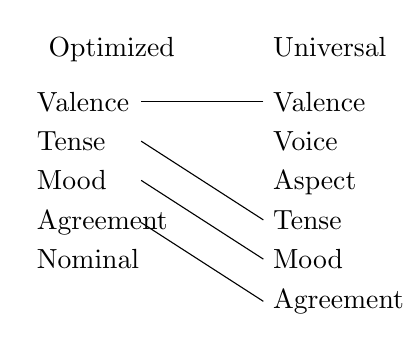
\begin{tikzpicture}[%
% common options for blocks:
block/.style = {draw, fill=blue!30, align=center, anchor=west,
            minimum height=0.65cm, inner sep=0},
% common options for the circles:
ball/.style = {circle, draw, align=center, anchor=north, inner sep=0}]
\node[rectangle,text width=1.2cm,anchor=base] (A0) at (4,-0.3) {Universal};
\node[rectangle,text width=0.9cm,anchor=base] (B0) at (1,-0.3) {Optimized};
\node[rectangle,text width=1.2cm,anchor=base] (A1) at (4,-1.0) {Valence};
\node[rectangle,text width=1.2cm,anchor=base] (A2) at (4,-1.5) {Voice};
\node[rectangle,text width=1.2cm,anchor=base] (A3) at (4,-2.0) {Aspect};
\node[rectangle,text width=1.2cm,anchor=base] (A4) at (4,-2.5) {Tense};
\node[rectangle,text width=1.2cm,anchor=base] (A5) at (4,-3.0) {Mood};
\node[rectangle,text width=1.2cm,anchor=base] (A6) at (4,-3.5) {Agreement};
\node[rectangle,text width=1.2cm,anchor=base] (B1) at (1,-1.0) {Valence};
\node[rectangle,text width=1.2cm,anchor=base] (B2) at (1,-1.5) {Tense};
\node[rectangle,text width=1.2cm,anchor=base] (B3) at (1,-2.0) {Mood};
\node[rectangle,text width=1.2cm,anchor=base] (B4) at (1,-2.5) {Agreement};
\node[rectangle,text width=1.2cm,anchor=base] (B5) at (1,-3.0) {Nominal};
\draw[-] (A1.west) to (B1.east);
\draw[-] (A4.west) to (B2.east);
\draw[-] (A5.west) to (B3.east);
\draw[-] (A6.west) to (B4.east);
\end{tikzpicture}

    \end{minipage}
        &
    \begin{minipage}{.3\textwidth}
    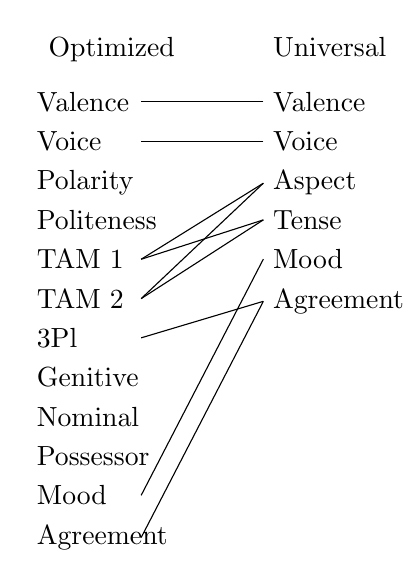
\begin{tikzpicture}[%
% common options for blocks:
block/.style = {draw, fill=blue!30, align=center, anchor=west,
            minimum height=0.65cm, inner sep=0},
% common options for the circles:
ball/.style = {circle, draw, align=center, anchor=north, inner sep=0}]
\node[rectangle,text width=1.2cm,anchor=base] (A0) at (4,-0.3) {Universal};
\node[rectangle,text width=0.9cm,anchor=base] (B0) at (1,-0.3) {Optimized};
\node[rectangle,text width=1.2cm,anchor=base] (A1) at (4,-1.0) {Valence};
\node[rectangle,text width=1.2cm,anchor=base] (A2) at (4,-1.5) {Voice};
\node[rectangle,text width=1.2cm,anchor=base] (A3) at (4,-2.0) {Aspect};
\node[rectangle,text width=1.2cm,anchor=base] (A4) at (4,-2.5) {Tense};
\node[rectangle,text width=1.2cm,anchor=base] (A5) at (4,-3.0) {Mood};
\node[rectangle,text width=1.2cm,anchor=base] (A6) at (4,-3.5) {Agreement};
\node[rectangle,text width=1.2cm,anchor=base] (B1) at (1,-1.0) {Valence};
\node[rectangle,text width=1.2cm,anchor=base] (B2) at (1,-1.5) {Voice};
\node[rectangle,text width=1.2cm,anchor=base] (B3) at (1,-2.0) {Polarity};
\node[rectangle,text width=1.2cm,anchor=base] (B4) at (1,-2.5) {Politeness};
\node[rectangle,text width=1.2cm,anchor=base] (B5) at (1,-3.0) {TAM 1};
\node[rectangle,text width=1.2cm,anchor=base] (B6) at (1,-3.5) {TAM 2};
\node[rectangle,text width=1.2cm,anchor=base] (B7) at (1,-4.0) {3Pl};
\node[rectangle,text width=1.2cm,anchor=base] (B8) at (1,-4.5) {Genitive};
\node[rectangle,text width=1.2cm,anchor=base] (B9) at (1,-5.0) {Nominal};
\node[rectangle,text width=1.2cm,anchor=base] (B10) at (1,-5.5) {Possessor};
\node[rectangle,text width=1.2cm,anchor=base] (B11) at (1,-6.0) {Mood};
\node[rectangle,text width=1.2cm,anchor=base] (B12) at (1,-6.5) {Agreement};
\draw[-] (A1.west) to (B1.east);
\draw[-] (A2.west) to (B2.east);
\draw[-] (A3.west) to (B5.east);
\draw[-] (A4.west) to (B5.east);
\draw[-] (A3.west) to (B6.east);
\draw[-] (A4.west) to (B6.east);
\draw[-] (A6.west) to (B7.east);
\draw[-] (A5.west) to (B11.east);
\draw[-] (A6.west) to (B12.east);
\end{tikzpicture}

    \end{minipage} 
    \\
    \textsc{Korean} & \textsc{Japanese} & \textsc{Sesotho Prefixes} \\
        \begin{minipage}{.3\textwidth}
    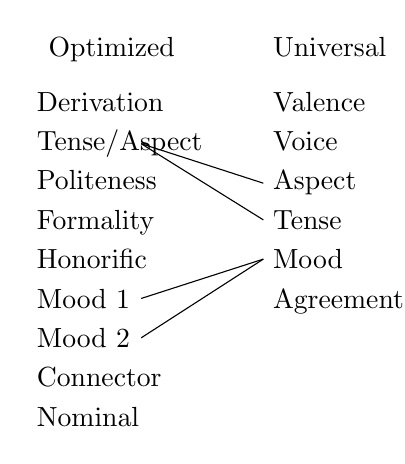
\begin{tikzpicture}[%
% common options for blocks:
block/.style = {draw, fill=blue!30, align=center, anchor=west,
            minimum height=0.65cm, inner sep=0},
% common options for the circles:
ball/.style = {circle, draw, align=center, anchor=north, inner sep=0}]
\node[rectangle,text width=1.2cm,anchor=base] (A0) at (4,-0.3) {Universal};
\node[rectangle,text width=0.9cm,anchor=base] (B0) at (1,-0.3) {Optimized};
\node[rectangle,text width=1.2cm,anchor=base] (A1) at (4,-1.0) {Valence};
\node[rectangle,text width=1.2cm,anchor=base] (A2) at (4,-1.5) {Voice};
\node[rectangle,text width=1.2cm,anchor=base] (A3) at (4,-2.0) {Aspect};
\node[rectangle,text width=1.2cm,anchor=base] (A4) at (4,-2.5) {Tense};
\node[rectangle,text width=1.2cm,anchor=base] (A5) at (4,-3.0) {Mood};
\node[rectangle,text width=1.2cm,anchor=base] (A6) at (4,-3.5) {Agreement};
\node[rectangle,text width=1.2cm,anchor=base] (B1) at (1,-1.0) {Derivation};
\node[rectangle,text width=1.2cm,anchor=base] (B2) at (1,-1.5) {Tense/Aspect};
\node[rectangle,text width=1.2cm,anchor=base] (B3) at (1,-2.0) {Politeness};
\node[rectangle,text width=1.2cm,anchor=base] (B4) at (1,-2.5) {Formality};
\node[rectangle,text width=1.2cm,anchor=base] (B5) at (1,-3.0) {Honorific};
\node[rectangle,text width=1.2cm,anchor=base] (B6) at (1,-3.5) {Mood 1};
\node[rectangle,text width=1.2cm,anchor=base] (B7) at (1,-4.0) {Mood 2};
\node[rectangle,text width=1.2cm,anchor=base] (B8) at (1,-4.5) {Connector};
\node[rectangle,text width=1.2cm,anchor=base] (B9) at (1,-5.0) {Nominal};
\draw[-] (A3.west) to (B2.east);
\draw[-] (A4.west) to (B2.east);
\draw[-] (A5.west) to (B6.east);
\draw[-] (A5.west) to (B7.east);
\end{tikzpicture}

    \end{minipage}
    &
    \begin{minipage}{.3\textwidth}
    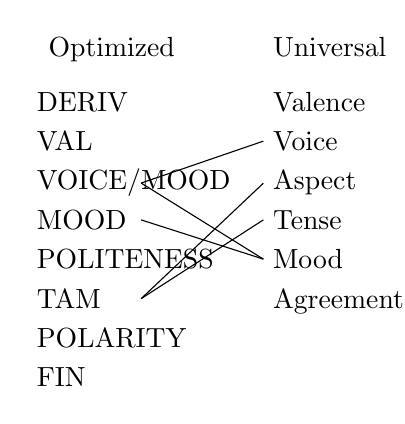
\begin{tikzpicture}[%
% common options for blocks:
block/.style = {draw, fill=blue!30, align=center, anchor=west,
            minimum height=0.65cm, inner sep=0},
% common options for the circles:
ball/.style = {circle, draw, align=center, anchor=north, inner sep=0}]
\node[rectangle,text width=1.2cm,anchor=base] (A0) at (4,-0.3) {Universal};
\node[rectangle,text width=0.9cm,anchor=base] (B0) at (1,-0.3) {Optimized};
\node[rectangle,text width=1.2cm,anchor=base] (A1) at (4,-1.0) {Valence};
\node[rectangle,text width=1.2cm,anchor=base] (A2) at (4,-1.5) {Voice};
\node[rectangle,text width=1.2cm,anchor=base] (A3) at (4,-2.0) {Aspect};
\node[rectangle,text width=1.2cm,anchor=base] (A4) at (4,-2.5) {Tense};
\node[rectangle,text width=1.2cm,anchor=base] (A5) at (4,-3.0) {Mood};
\node[rectangle,text width=1.2cm,anchor=base] (A6) at (4,-3.5) {Agreement};
\node[rectangle,text width=1.2cm,anchor=base] (B1) at (1,-1.0) {DERIV};
\node[rectangle,text width=1.2cm,anchor=base] (B2) at (1,-1.5) {VAL};
\node[rectangle,text width=1.2cm,anchor=base] (B3) at (1,-2.0) {VOICE/MOOD};
\node[rectangle,text width=1.2cm,anchor=base] (B4) at (1,-2.5) {MOOD};
\node[rectangle,text width=1.2cm,anchor=base] (B5) at (1,-3.0) {POLITENESS};
\node[rectangle,text width=1.2cm,anchor=base] (B6) at (1,-3.5) {TAM};
\node[rectangle,text width=1.2cm,anchor=base] (B7) at (1,-4.0) {POLARITY};
\node[rectangle,text width=1.2cm,anchor=base] (B8) at (1,-4.5) {FIN};
\draw[-] (A2.west) to (B3.east);
\draw[-] (A5.west) to (B3.east);
\draw[-] (A5.west) to (B4.east);
\draw[-] (A3.west) to (B6.east);
\draw[-] (A4.west) to (B6.east);
\end{tikzpicture}

    \end{minipage}
        &
    \begin{minipage}{.3\textwidth}
    \begin{tikzpicture}[%
% common options for blocks:
block/.style = {draw, fill=blue!30, align=center, anchor=west,
            minimum height=0.65cm, inner sep=0},
% common options for the circles:
ball/.style = {circle, draw, align=center, anchor=north, inner sep=0}]
\node[rectangle,text width=1.2cm,anchor=base] (A0) at (4,-0.3) {Universal};
\node[rectangle,text width=0.9cm,anchor=base] (B0) at (1,-0.3) {Optimized};
\node[rectangle,text width=1.2cm,anchor=base] (A1) at (4,-1.0) {Valence};
\node[rectangle,text width=1.2cm,anchor=base] (A2) at (4,-1.5) {Voice};
\node[rectangle,text width=1.2cm,anchor=base] (A3) at (4,-2.0) {Aspect};
\node[rectangle,text width=1.2cm,anchor=base] (A4) at (4,-2.5) {Tense};
\node[rectangle,text width=1.2cm,anchor=base] (A5) at (4,-3.0) {Mood};
\node[rectangle,text width=1.2cm,anchor=base] (A6) at (4,-3.5) {Agreement};
\node[rectangle,text width=1.2cm,anchor=base] (B1) at (1,-1.0) {Other_6};
\node[rectangle,text width=1.2cm,anchor=base] (B2) at (1,-1.5) {Other_2a};
\node[rectangle,text width=1.2cm,anchor=base] (B3) at (1,-2.0) {Infinitive};
\node[rectangle,text width=1.2cm,anchor=base] (B4) at (1,-2.5) {Other_ij};
\node[rectangle,text width=1.2cm,anchor=base] (B5) at (1,-3.0) {Other_wo};
\node[rectangle,text width=1.2cm,anchor=base] (B6) at (1,-3.5) {Other_di};
\node[rectangle,text width=1.2cm,anchor=base] (B7) at (1,-4.0) {Other_copula};
\node[rectangle,text width=1.2cm,anchor=base] (B8) at (1,-4.5) {Other_1s};
\node[rectangle,text width=1.2cm,anchor=base] (B9) at (1,-5.0) {Other_lo};
\node[rectangle,text width=1.2cm,anchor=base] (B10) at (1,-5.5) {Subject};
\node[rectangle,text width=1.2cm,anchor=base] (B11) at (1,-6.0) {Other_f^};
\node[rectangle,text width=1.2cm,anchor=base] (B12) at (1,-6.5) {Other_2};
\node[rectangle,text width=1.2cm,anchor=base] (B13) at (1,-7.0) {Tense/aspect};
\node[rectangle,text width=1.2cm,anchor=base] (B14) at (1,-7.5) {Int/Rel};
\node[rectangle,text width=1.2cm,anchor=base] (B15) at (1,-8.0) {Other_av};
\node[rectangle,text width=1.2cm,anchor=base] (B16) at (1,-8.5) {Negation};
\node[rectangle,text width=1.2cm,anchor=base] (B17) at (1,-9.0) {Other_9};
\node[rectangle,text width=1.2cm,anchor=base] (B18) at (1,-9.5) {Other_3};
\node[rectangle,text width=1.2cm,anchor=base] (B19) at (1,-10.0) {Other_17};
\node[rectangle,text width=1.2cm,anchor=base] (B20) at (1,-10.5) {Other_10};
\node[rectangle,text width=1.2cm,anchor=base] (B21) at (1,-11.0) {Other_7};
\node[rectangle,text width=1.2cm,anchor=base] (B22) at (1,-11.5) {Other_pr};
\node[rectangle,text width=1.2cm,anchor=base] (B23) at (1,-12.0) {Object/reflexive};
\draw[-] (A6.west) to (B10.east);
\draw[-] (A3.west) to (B13.east);
\draw[-] (A4.west) to (B13.east);
\draw[-] (A1.west) to (B23.east);
\end{tikzpicture}

    \end{minipage}
    \\
    \textsc{Sesotho Suffixes} \\
        \begin{minipage}{.3\textwidth}
    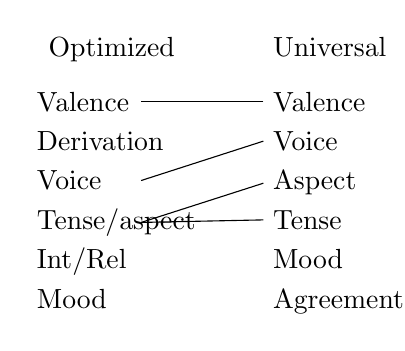
\begin{tikzpicture}[%
% common options for blocks:
block/.style = {draw, fill=blue!30, align=center, anchor=west,
            minimum height=0.65cm, inner sep=0},
% common options for the circles:
ball/.style = {circle, draw, align=center, anchor=north, inner sep=0}]
\node[rectangle,text width=1.2cm,anchor=base] (A0) at (4,-0.3) {Universal};
\node[rectangle,text width=0.9cm,anchor=base] (B0) at (1,-0.3) {Optimized};
\node[rectangle,text width=1.2cm,anchor=base] (A1) at (4,-1.0) {Valence};
\node[rectangle,text width=1.2cm,anchor=base] (A2) at (4,-1.5) {Voice};
\node[rectangle,text width=1.2cm,anchor=base] (A3) at (4,-2.0) {Aspect};
\node[rectangle,text width=1.2cm,anchor=base] (A4) at (4,-2.5) {Tense};
\node[rectangle,text width=1.2cm,anchor=base] (A5) at (4,-3.0) {Mood};
\node[rectangle,text width=1.2cm,anchor=base] (A6) at (4,-3.5) {Agreement};
\node[rectangle,text width=1.2cm,anchor=base] (B1) at (1,-1.0) {Valence};
\node[rectangle,text width=1.2cm,anchor=base] (B2) at (1,-1.5) {Derivation};
\node[rectangle,text width=1.2cm,anchor=base] (B3) at (1,-2.0) {Voice};
\node[rectangle,text width=1.2cm,anchor=base] (B4) at (1,-2.5) {Tense/aspect};
\node[rectangle,text width=1.2cm,anchor=base] (B5) at (1,-3.0) {Int/Rel};
\node[rectangle,text width=1.2cm,anchor=base] (B6) at (1,-3.5) {Mood};
\draw[-] (A1.west) to (B1.east);
\draw[-] (A2.west) to (B3.east);
\draw[-] (A3.west) to (B4.east);
\draw[-] (A4.west) to (B4.east);
\end{tikzpicture}

    \end{minipage}
\end{tabular}
    \caption{Comparing optimized orders of verb affixes with the universal ordering described by \citep{bybee-morphology-1985}. \mhahn{It might be possible to remove this figure and instead indicate the match by introducing color coding to Figure 8, so it would become visually obvious there. What do you think?}}
    \label{fig:optimized_and_universal_orders}
\end{figure}



\begin{table}[]
    \centering
    \begin{tabular}{l|l|l|ll|ll|llllll}
%    &     &    \multicolumn{2}{c|}{Pairs} & \multicolumn{2}{c|}{Full} & \multicolumn{2}{c}{Full (Types)} \\
%      &   &     Optim. & Baseline & Quantile. & 95\% CI  & Optim. & Baseline \\ \hline
%     &   &     Optim. & Baseline & Quantile  \\ \hline
     &   &     Optim. & \multicolumn{2}{|c}{Baseline (Random)} & \multicolumn{2}{|c|}{Baseline (Universals)}  \\ 
     &  &            & Accuracy & Quantile & Accuracy & Quantile \\
     \hline
     \multirow{3}{*}{Nouns} & Finnish & 1.0 (0.0) & 0.52 (0.32) & 1.0  [0.95, 1.0]  \\
 & Turkish & 1.0 (0.0) & 0.54 (0.36) & 1.0  [0.95, 1.0]  \\
 & Hungarian & 1.0 (0.0) & 0.47 (0.37) & 1.0  [0.95, 1.0]  \\
\hline
\multirow{7}{*}{Verbs} & Finnish & 0.4 (0.3) & 0.57 (0.38) & 0.43  [0.34, 0.52]  \\
 & Hungarian & 0.95 (0.09) & 0.52 (0.4) & 0.81  [0.72, 0.88]  \\
 & Turkish & 0.96 (0.09) & 0.52 (0.14) & 1.0  [0.96, 1.0]  \\
 & Korean & 0.97 (0.1) & 0.55 (0.24) & 1.0  [0.95, 1.0]  \\
 & Japanese & 0.95 (0.0) & 0.48 (0.24) & 1.0  [0.85, 1.0]  \\
 & Sesotho (P) & 0.98 (0.0) & 0.56 (0.48) & 0.77  [0.65, 0.86]  \\
 & Sesotho (S) & 0.62 (0.0) & 0.43 (0.23) & 0.82  [0.72, 0.9]  \\

    \end{tabular}
    \caption{Accuracies in predicting morpheme ordering. `Optim.' indicates grammars optimized for AUC, `'Baseline' indicates randomly constructed weights.
    In each cell, we provide the mean and the standard deviation over orderings.
    We also show the fraction of baseline orderings with lower accuracy than the optimized order, with a 95\% binomial confidence interval.
    \mhahn{could think about making this a set of small violin plots for each language, instead of providing numerical hard-to-think-about quantile information}
    }
    \label{tab:optimized_acc}
\end{table}















\subsection{Relation to previous accounts}



\paragraph{Relation to Previous Theories} here explain link to bybee

We suggest that mutual information provides an operational formalization of semantic relevance. \becky{Should this be explained earlier in the paper?}
For instance, we expect that passive markers have a high mutual information with the verb stem, since only certain verbs (typically a subclass of the transitive verbs) can form a passive.
The idea that mutual information is an operationalization of semantic closeness has also been suggested in other places; for instance, \citep{culbertson2020from} link mutual information to conceptual closeness as a driving factor of noun phrase modification.

\mhahn{I'm pondering to what extent it would be helpful to expound on the connection between the tradeoff and locality, to make the link to Bybee.} \jd{i think it would be very helpful. currently the connection to bybee feels a little off the cuff and unmotivated. it would be worth being more explicit about bybee's notion of relevance, and why we think MI is a good formalization of it.}




%\subsubsection{Semantic Scope; Syntactic Structure; Historical Development}
%Morpheme ordering has been described from the perspective 
%Besides the explanation of broad typological tendencies, which we are interested in here, the linguistic literature has also debated at which level of linguistic representation morpheme ordering should be described, proposing accounts located at different levels such as the syntax-phonology interface \citep{baker1985the} and an autonomous layer of morphological description \citep{hyman2003suffix}.
%TODO also template vs scope vs...
%We do not see the memory--surprisal tradeoff as competing with or contradicting these studies.
%Rather, it specifies tendencies for ordering that could be implemented at different levels of linguistic description.

%\paragraph{Revelance and Proximity}


%A related family of explanations holds that those affixes are closest to the root that are most relevant to the root.
%Our optimized orders of Turkish and Hungarian \becky{Are there other languages?} perfectly match Bybee's proposed universal verbal inflection ordering (Figure REF).
%This suggests that high mutual information generally correlates with semantic relevance. 


In this section, we relate our results to existing explanatory accounts of morpheme ordering.
In a review of research on morpheme ordering, \citet{manova2010modeling} % https://homepage.univie.ac.at/stela.manova/modeling%20affix%20order.pdf
categorize approaches to morpheme ordering into three classes (similarly \citet{rice2000morpheme, rice2011principles}): orderings that are motivated by properties of syntax, semantics or phonology; orderings that are motivated by human language processing responding to statistical properties of language; and orderings that are arbitrarily stipulated.
%Our approach falls into the second class, explaining morpheme ordering based on minimization of human processing effort.
In this section, we describe how our account relates to other accounts across these three \becky{four?} clusters, and show how the memory-surprisal tradeoff has tight connections with notions proposed across seemingly very different accounts.

%\mhahn{One can debate whether this trichotony is right -- e.g. Bybee's approach could be thought of as cognitive. What the second class 


%- citing \cite{rice2000morpheme}; Manova and Aronoff 2010; Saarinen and Hay 2014
%Rice states three types of explanations/phenomena:
%- extra-grammatical: frequency, productivity, parsability


\subsubsection{Relations to Syntactic Theories}

A family of theories hold that morpheme ordering is motivated by constraints placed on morphology through the interaction with other aspects of grammar.
The approaches most relevant for our results are approaches in terms of the relation of morphology to syntax~\citep{baker1985the} and semantics~\citep{bybee-morphology-1985,rice2000morpheme}.

%- grammatuical principle (syntactic, semantic, phonological). famous examples Mirror Principle and Bybee's relevance Principle; Scope (Rice)


%Mirror princuiple built into Distributed Morphology (Harley and Noyer 1998)

%\mhahn{report the following somewhere}
%We measured the mutual information between roots and features using the other Universal Dependencies corpora for which these features were available.
%First, for nouns, we compared the mutual information between the lemma and case and number, using a mixed-effects model with random effects for languages and language families.
%Across 34 languages, mutual information tended to be higher for number than for case ($\beta=0.04$, $SE=0.015$, $t=2.58$, 30 languages).
%For verbs, we compared mutual information between the root and voice, TAM, and subject agreement features.
%Mutual information was higher for TAM than for agreement ($\beta=0.1$, $SE=0.04$, $t=2.29$, 37 languages), however, there was no significant difference between TAM and voice ($\beta=0.08$, $SE=0.058$, $t=1.39$, 30 languages).


%TODO think about where to explain this As mentioned in section \becky{cite S2}, Bybee proposes a concept of \textit{semantic relevance}, which is the degree to which one morpheme affects the semantic content of the other \becky{cite bybee}. She hypothesizes that morphemes that are more highly relevant to each other should be closer to each other, and therefore proposes a universal ordering of verbal inflectional morphemes. For example, attaching a causative marker to a root meaning "to die" produces a verb form meaning "to kill." Since the causative greatly changes the semantic content of the original root, the causative is highly relevant to the root. 
%\becky{Format Korean example of juk-da ``to die" and juk-i-da ``to kill"}
%Bybee did not provide a way to computationally measure semantic relevance. 


%Other explanations suggest that morphemes are ordered based on (TODO CITE).
%The most straightforwardly related account is that of Bybee (1985) Semantic relevance
%CARP template in Bantu
%Explanations for the orders

%talk about Relevance and Mutual Information
%\paragraph{Morphemes as Fossilized Words}\

It has long been observed that the ordering of morphemes often parallels the order of independent words of corresponding meanings \citep{givon1971historical,venneman1973explanation,baker1985the}.
One explanation for this is that the ordering of morphemes reflects the order of formerly independent elements that have been fossilized into bound morphemes, which can often be verified in languages where historical data is available \citep{givon1971historical,venneman1973explanation}.
% interesting: Evans, Nicholas (1995). Multiple case in Kayardild: Anti-iconic suffix ordering and the diachronic filter. In Plank (ed.) 1995, 396-430. 
% Moravcsik, Edith A. (1995). Summing up Suffixaufnahme. In Plank (ed.) 1995, 451-484.  HEREL : 478, G24
% Cited by https://typo.uni-konstanz.de/rara/universals-archive/41/
On the other hand, \citet{bybee-morphology-1985} points out that there are historically documented cases where morpheme ordering has been restructured in ways that do not reflect former independent words, but respect the universal tendencies proposed by her \becky{``that she proposed" instead of ``proposed by her" ?} (see also \citet{mithun2000the, haspelmath1993the, mithun1995affixation}; \citet[Section 15]{rice2000morpheme}).
A correspondence between the ordering of words and morphemes has also been postulated on a purely synchronic basis as a constraint on possible human languages.
\cite{baker1985the} proposed the Mirror Principle, which -- informally -- states that the order of elements (morphemes) in morphology reflects the order of elements (words) in syntax.
A large body of work in theoretical syntax describes word and morpheme ordering using the same processes and principles \citep{halle1993distributed}.
As a theory of ordering at multiple levels, the Efficient Tradeoff Hypothesis is compatible with these different historical paths and predicts these ordering patterns independently of the historical path leading to the morphemes found in a given language.



%As the memory-surprisal tradeoff is optimized by word order, this is compatible with our results:
%To the extent that morpheme order does reflect fossilized word order, morpheme order should continue to reflect optimization for the tradeoff.


%To the extent that similar statistical patterns of usage hold for corresponding words and morphemes, this again is compatible with the Efficient Tradeoff Hypothesis.

%\mhahn{TODO regarding scope: \citep{baker1988incorporation,foley1984functional,chierchia1990meaning,valin1992a}}


%This can be related to the scope-based explanation to the extent that syntactic structure and word order reflect scope.
% INTERESTING reference: http://www.jzeller.de/pdf/CARP.pdf

%\paragraph{Semantic Scope}


%Description in terms of scope faces limitations when order is different from semantic scope.
%\cite{Hyman2003}
%Hyman  (2003:  249) proposed the CARP template to describe suffix order in Bantu languages (such as Sesotho), a templatic order for valence and voice morphemes that can be different from scope order.
%In \cite{Hyman2003}'s model, order is determined based on both the CARP template and a preference for ismorphism with semantic scope.
%


%The principle of semantic scope is explained in detail and illustrated with copiousexamples in \cite{caballero2010scope}. \cite{narrog2010the} and most of the papers included in thenext issue provide analyses based on semantic scope, Aronoff and Xu (next issue),Korotkova and Lander (next issue), and Nordlinger (next issue).




Other prominent accounts are in terms of a correspondence between morpheme ordering and semantics~\citep{bybee-morphology-1985,rice2000morpheme}.
\citet{bybee-morphology-1985} argues that semantic relevance determines ordering.
For example, morphemes changing a verb's argument structure, such as passives and causatives, have a particularly strong relation to the verb's semantics, as they fundamentally alter the nature of the event described, whereas tense or agreement markers are much less tightly linked the the verb's meaning.
We suggest that mutual information provides an operational formalization of semantic relevance. \becky{Should this be explained earlier in the paper?}
For instance, we expect that passive markers have a high mutual information with the verb stem, since only certain verbs (typically a subclass of the transitive verbs) can form a passive.
The idea that mutual information is an operationalization of semantic closeness has also been suggested in other places; for instance, \citep{culbertson2020from} link mutual information to conceptual closeness as a driving factor of noun phrase modification.

A second prominent semantic account is in terms of semantic scope \citep{rice2000morpheme}.
This is the idea that morphemes are ordered in the order in which their meanings combine \citep[e.g.,][]{rice2000morpheme, caballero2010scope,  narrog2010the, korotkova2010deriving}.
The relative ordering of valence and voice is a good example for the scope-based explanation.
Valence affixes change the number of arguments, and passive (voice) promotes one argument to the subject position.
This can affect an argument introduced by a voice marker.
The following example from Turkish illustrates this (\cite{schaaik2020turkish}, section 30.8.2):


\begin{tabular}{ccccccc}
don-dur-ul & freeze-caus-pass & be frozen \\
don-dur & freeze-caus & to freeze (something) \\
don & freeze& to freeze \\
\end{tabular}

Turkish has suffixes both for causative and passive.
When adding both suffixes simultaneously, the causative marker appears closer to the root.
This corresponds to the order in which the meanings of these suffixes combine with the meaning of the root:
Causative adds an argument indicating who makes an object freeze, and passive then removes that argument, yielding a verb describing something that is being frozen by someone.

A priori, semantic scope is different from mutual information.
However, there are arguments that scope relations correlate with mutual information.
\citet{culbertson2020from} made a related argument for the order of nominal modifiers as in ``the four green books'', where mutual information predicts the order of attachment of modifiers to the noun.
%Furthermore, if the semantic propositions that speakers communicate are modeled using a probabilistic language-of-thought grammar such as mutual information will also correlate with scope ordering (see SI Appendix Section S4 for a simulation study).




\subsubsection{Motivations in Terms of Human Language Processing}

A prominent cognitively-motivated theory of morpheme ordering is the theory of Complexity-Based Ordering \citep{hay2002speech,plag2002the,hay2004what,hay2005shifting,plag2009suffix}.
This theory holds that affixes are closer to the root when they are less ``separable'', where separability indicates the productivity of an affix and the likelihood that affixes are processed separately with the base in human lexical access  \citep{baayen1993on}.
%In particular, affixes are less ``separable'' when they are processed holistically together with the base in human lexical access \citep{baayen1993on}. %, such as in the dual processing race model of morphological access, which asserts that morphological forms can be processed either separately in terms of its components or as a whole \citep{baayen1993on}.
%Forms are more separable if they are less likely to be processed together with the root (Baayen \& Schreuder 1999, Baayen \& Moscoso del Prado Mart ́ın 2005).
%also mention \cite{manova2010suffix}
%\cite{plag2009suffix} %http://www.sfs.uni-tuebingen.de/~hbaayen/publications/plagBaayenLanguage2009.pdf
A statistical operationalization of separability is in terms of relative frequencies:
affixes are more likely to be processed together with the root when the composite form has a higher frequency compared to the base form \citep{hay2001lexical}. % , lee2011ordering
This has an interesting relation to mutual information: 
If the compound form is very frequent, in relation to the baseline frequencies of the base and the affix, then there is high (pointwise) mutual information between them.
\mhahn{Make clear that this theory hasn't been applied to the kinds of affix orderin generalizations that we look at in this paper.}

Most closely related to our proposal, \citet{inkelas2016affix} proposed that morphemes are ordered together when they are informative about each other.
They considered a notion of informativity introduced by \citet{priva2017informativity}, which is different from but related to the mutual information between adjacent morphemes $I_1$ (see SI Appendix Section S3 for details).
%Formally (drawing on the notion of informativity defined by \citet{priva2017informativity}), they considered the informativity between a suffix $S_i$ and the preceding $S_{i-1}$ as 
%\begin{equation}
%    \sum_{S_{i-1}, S_{i}} \frac{P(S_{i-1} , S_i)}{P(S_i)} \log P(S_i | S_{i-1})
%\end{equation}
They tested this idea in a pilot study of Turkish, finding that high-informativity suffixes are closer to the root.
%This notion of informativity is similar to $I_1$, only differing in whether the $P(S_i)$ term occurs inside the logarithm:
%\begin{equation}
%   I_1 = \sum_{S_{i-1}, S_{i}} P(S_{i-1} , S_i) \log \frac{P(S_i | S_{i-1})}{P(S_i)}
%\end{equation}


%Inkelas: informativity: they propose that bigram surprisal is minimized (not their terminology), test this in a pilot study of Turkish, with partially confirming results \citep{inkelas2015informativity}
%Alternatively, the lower thefrequency of the derived word in relation to the base word, the more important the role ofthe constituents become
%Hay and Plag (2004) show that ordering correlates with relative frequency and productivity
%Hay (in press) distinguishes between derived forms which are more frequent than the bases they contain (e.g.illegible is more frequent than legible), and derived forms whic hare less frequent than their bases (e.g.illiberal is less frequent than liberal).
% argues that whether an affix is processed together with the root is determined in part by the relative frequency
%\begin{equation}
%    \frac{P(base+affix)}{P(base)}
%\end{equation}
%\begin{equation}
%    \log \frac{P(base, affix)}{P(base)} = \log P(affix|base)
%\end{equation}
%\begin{equation}
%    pmi(base, affix) = \log \frac{p(affix|base)}{p(base)}
%\end{equation}
%Hay and Baayen (2002).
%Hay and Plag (2004): parsing ratio and productivity measured by Hay and Baayen (2002).
%Complexity-based Ordering, the position of a given suffix inthe hierarchy reflects the degree to which that suffix is processed independently of its base.

%\citet{hay2004what} propose a model of complexity-based ordering based on processing considerations, called complexity-based ordering, arguing that affixes are further away from the root when they can be separated more easily in processing, testing this theory using 15 English affixes.


%from Inkelas



\subsubsection{Arbitrary Orderings}

There are also studies suggesting language-specific and essentially arbitrary properties of morpheme ordering.
A classical approach to describing morpheme ordering is in terms of levels, where morphemes from a higher level occur before morphemes from a lower level \citep{siegel1979topics}, and in terms of templates that describe the ordering of morphemes \citep{simpson1986pronominal,spencer1991morphological,stump1992on,inkelas1993nimboran,hyman2003suffix,nordlinger2010verbal}.
Ordering based on language-specific templates has been proposed specifically in cases where observed morpheme ordering is in conflict with semantic scope, as in Bantu languages \citep{hyman2003suffix}.
\citet{fabb1988english} prominently describes English affix ordering in terms of the selectional restrictions that individual affixes place on which other affixes they can attach to.
While this approach does not make statements as to which affixes would go closer to the base in a given language, it does suggest that morpheme ordering is described based on the pairwise interactions between adjacent morphemes.
In a similar vein, \citet{ryan2010variable} propose a model based on weighted bigram constraints in Tagalog, for the (rather uncommon) case of flexible morpheme ordering.
Ordering constraints operating on adjacent pairs of morphemes might provide relatively efficient memory-surprisal tradeoffs because the appearance of a morpheme is constrained only by its immediately adjacent morphemes.




%Tension between Scope and templatic: \citep{hyman2003suffix}; \cite{aronoff2010introduction}; \cite{spencer2003putting}
%- arbitrary language-specific tenplatic (Fabb 1988 English affix ordering; position class templates, Simpson and Withgott 1986) (also finite-state automata Hankamer 1986; Karttunen 2003) 

%re scope also \cite{alsina1999where}

%\cite{manova2010modeling} % https://homepage.univie.ac.at/stela.manova/modeling%20affix%20order.pdf
%also provide a ctagoeirzation into grammatical, psycholinguistic, unmotivated (among others)





%\cite{aronoff2010a} % Within this model, phonological form is spelled out by means of individual-language-particular realization constraints that associate abstract morphosyntactic feature values with phonological forms and that are ordered among more general constraints governing factors like scope and feature splitting. The data used to exemplify the application of our theory to affix order are drawn from Haspelmath’s (A grammar of Lezgian, Mouton de Gruyter, Berlin, 1993) grammar of Lezgian, a language of the Northeast Caucasian family spoken largely in Dagestan (Russia) and Azerbaijan.



%\paragraph{Templates}
%CARP template
%\cite{muysken1981quechua}
%\cite{mccarthy2008generalized} phonology
%\cite{hyman2003suffix}
%\cite{kanu2009suffix} morphotactics, not semantic scope





%\subsubsection{Semantic Scope; Syntactic Structure; Historical Development}
%Morpheme ordering has been described from the perspective 
%Besides the explanation of broad typological tendencies, which we are interested in here, the linguistic literature has also debated at which level of linguistic representation morpheme ordering should be described, proposing accounts located at different levels such as the syntax-phonology interface \citep{baker1985the} and an autonomous layer of morphological description \citep{hyman2003suffix}.
%TODO also template vs scope vs...
%We do not see the memory--surprisal tradeoff as competing with or contradicting these studies.
%Rather, it specifies tendencies for ordering that could be implemented at different levels of linguistic description.

%\paragraph{Revelance and Proximity}


%A related family of explanations holds that those affixes are closest to the root that are most relevant to the root.
%Our optimized orders of Turkish and Hungarian \becky{Are there other languages?} perfectly match Bybee's proposed universal verbal inflection order (Figure REF).
%This suggests that high mutual information generally correlates with semantic relevance. 